% !TeX spellcheck = es_ES

% Funcionamento e uso de un CVS: Git
\title[Git e GitHub]{Control de versións Git}
\author[Fran Rúa e Breixo Camiña]{}

\section{Control de versións Git}
\label{sec:Git}

\begin{frame}
  \titlepage
  \begin{figure}[H]
    \centering
    
\includegraphics[width=0.5\linewidth]{logo-git}
    \label{fig:logo-git}
  \end{figure}
\end{frame}

\begin{frame}
  \frametitle{Táboa de contidos}
  \tableofcontents[currentsection]
\end{frame}

\subsection{Sistema de control de versións}
\label{subsec:vcs}
\begin{frame}{Sistema de control de versións}
  \begin{block}{¿Que é o control de versións?}
    É a xestión de diversos cambios que se realizan sobre os elementos de algún produto ou unha configuración do mesmo. Unha versión é o estado no que se encontra o produto nun momento do seu desenvolvemento.
  \end{block}
  \begin{block}{¿Que é un sistema de control de versións?}
    Son ferramentas que facilitan a administración das distintas versións de cada produto desenvolvido.
  \end{block}
\end{frame}

\subsection{¿Que é Git?}
\begin{frame}
  \frametitle{¿Que é Git?}
  \begin{block}{Definición}
    Git é un sistema de control de versións distribuido gratuito e de código aberto deseñado para xestionar todo dende un proxecto pequeno a un moi grande, de forma rápida e eficiente.
  \end{block}
  \begin{itemize}
  \item É rápido, eficiente, escalable e distribuido.
  \item Propicia o traballo en local e o uso de ramas.
  \item Proporciona un nivel de historia do proxecto completísimo.
  \item Diferencia os commits unívocamente mediante claves xeradas con SHA-1.
  \item Cumpre as palabras máxicas do GPUL: é libre e gratuito.
  \end{itemize}
\end{frame}

\subsection{Comparación con outros servizos}
\begin{frame}
  \scriptsize
  \frametitle{Comparación con servizos de almacenamento na nube}
  \begin{multicols}{2}
    \textbf{Dropbox:}
    \begin{itemize}
    \item Útiles para compartir ficheiros con compañeiros.
    \item O problema é se queres modificar o mesmo ficheiro ambos ó mesmo tempo, vai haber problemas de sincronización.
    \end{itemize}
    \columnbreak
    \textbf{Google Drive:}
    \begin{itemize}
    \item Útil para modificar ficheiros en tempo real, pero con proxectos software é imposible.
    \end{itemize}
  \end{multicols}
  \begin{alertblock}{VCS}
    Os VCS son a solución!
  \end{alertblock}
\end{frame}

\begin{frame}
  \frametitle{Comparación con outros VCS}
  \tiny
  \begin{multicols}{2}
    \textbf{Subversion:}
    \begin{itemize}
    \item Git é moito máis rápido e lixeiro que SVN (un repo SVN ocupa 30x o que un de Git).
    \item Unha rama en SVN é unha copia completa do repositorio mentres que en Git é un simple punteiro e conleva toda a historia do proxecto ata ese punto.
    \item Git proporciona mellor auditoría de eventos de ramificación e fusión (ramas e merge).
    \item SVN é usado en case todas as asignaturas da FIC.
    \item Por dicir algo bo de SVN, é máis fácil o seu uso para principiantes e ten máis ferramentas de integración con IDEs.
    \end{itemize}
    \begin{figure}
      \centering
      
\includegraphics[width=0.3\linewidth]{svn}
      \label{fig:svn}
    \end{figure}

    \columnbreak

    \textbf{Mercurial:}
    \begin{itemize}
    \item Máis fácil de aprender que Git.
    \item Mercurial blablabla
    \end{itemize}
    \begin{figure}
      \centering
      
\includegraphics[width=0.3\linewidth, height=0.2\textheight]{mercurial}
      \label{fig:mercurial}
    \end{figure}
  \end{multicols}
\end{frame}

\subsection{Instalación nos SO}
\begin{frame}
  \frametitle{Instalación nos SO}
  \begin{exampleblock}{Linux}
    (Proyecto Debian) apt-get install git\\
    (RPM) yum install git
  \end{exampleblock}
  \begin{block}{Mac}
    http://git-scm.com/download/mac
  \end{block}
  \begin{alertblock}{Windows}
    https://git-scm.com/download/win
  \end{alertblock}	
\end{frame}

\begin{frame}
  \frametitle{Interfaces gráficas de usuario para Git}
  \begin{exampleblock}{Linux}
    SmartGit - http://www.syntevo.com/smartgit/download
  \end{exampleblock}
  \begin{alertblock}{Mac e Windows}
    Sourcetree - https://es.atlassian.com/software/sourcetree/overview/
  \end{alertblock}
\end{frame}

\subsection{Inicio do uso de Git}
\begin{frame}[fragile]
  \frametitle{Inicio do uso de Git}
  \small
  Creamos unha carpeta no escritorio que lle chamaremos 'CharlaGit'.
  Dentro da carpeta, executamos \textbf{git init} e debería saír:
  \tiny
\begin{verbatim}
	breixocf@BreixoCF ~/Desktop/PruebasGit 6 $ git init 
	Initialized empty Git repository in /home/breixocf/Desktop/CharlaGit/.git/
\end{verbatim}
  \small
  Creouse unha carpeta .git que conterá todo o repositorio, que será a base de datos de Git.
  Antes de nada, imos configurar o noso repo, indicando o nome e correo do usuario con \textbf{git config}  e comprobamos os cambios.
  \tiny
\begin{verbatim}
	breixocf@BreixoCF ~/Desktop/CharlaGit 18 $ git config --global user.name "Breixo Camiña"
	breixocf@BreixoCF ~/Desktop/CharlaGit 19 $ git config --global user.email 
	breixocf@BreixoCF ~/Desktop/CharlaGit 21 $ git config --list 
	user.name=Breixo Camiña
	user.email=breixo.camina@udc.es
	core.repositoryformatversion=0
	core.filemode=true
	core.bare=false
	core.logallrefupdates=true
\end{verbatim}	
\end{frame}

\begin{frame}[fragile]
  \frametitle{Zonas de traballo de Git}
  \begin{multicols}{2}
    \begin{figure}
      \centering
      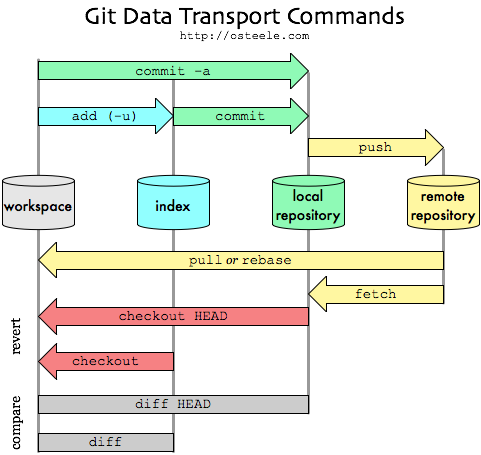
\includegraphics[width=1\linewidth]{flujo-git}
      \label{fig:flujo-git}
    \end{figure}
    \columnbreak
    \tiny
    \begin{itemize}
    \item Workspace: É onde están os ficheiros que actualmente non están en seguimento, é dicir, os que están na nosa zona de traballo.
    \item Index: É onde están as modificacións que se engadirán ó repo local. Os ficheiros están preparados para engadir ó repositorio local, pero aínda non están no historial do proxecto. 
    \item Local Repository: É onde están os ficheiros confirmados que conformarán unha versión nova do proxecto. Almacena os metadatos e a base de datos do proxecto. Tamén se lle chama HEAD.
    \item Remote Repository: Son os repositorios que estarán en internet, onde accederán varios usuarios...
    \end{itemize}
  \end{multicols}
\end{frame}

\begin{frame}[fragile]
  \frametitle{Primer comando: git status}
  \begin{block}{git status}
    Amosa o estado no que se atopan os ficheiros do repositorio.
  \end{block}
  Executando \textbf{git status} sobre o noso repositorio, debería aparecer a seguinte mensaxe:
  \tiny
\begin{verbatim}
	breixocf@BreixoCF ~/Desktop/CharlaGit 32 $ git status
	On branch master
	Initial commit
	nothing to commit (create/copy files and use "git add" to track)
\end{verbatim}
  \small Como todavía non hai ningún ficheiro en seguimento (pode haber milleiros de ficheiros na carpeta, pero non están sendo trackeados polo repositorio), dinos que usemos git add para engadir algún ficheiro a seguir.
\end{frame}

\begin{frame}[fragile]
  \frametitle{Segundo comando: git add}
  \begin{block}{git add}
    Engade un ficheiro da nosa zona de traballo ao índice, preparándoo para
    engadilo ó repositorio.
  \end{block}
  \small
  Creamos un ficheiro co comando \textbf{touch hola.txt} e executamos \textbf{git status} para ver o seu estado:
  \tiny
\begin{verbatim}
	breixocf@BreixoCF ~/Desktop/CharlaGit 32 $ git status
	On branch master
	Initial commit
	Untracked files:
	  (use "git add <file>..." to include in what will be committed)
	     hola.txt
	nothing added to commit but untracked files present (use "git add" to track)
\end{verbatim}
\end{frame}

\begin{frame}[fragile]
  \frametitle{Segundo comando: git add}
  O ficheiro non está en seguimento pese a estar na carpeta, é necesario executar o comando \textbf{git add} para iso. Así que agora executamos \textbf{git add} e indicamos o ficheiro que queremos engadir. Se queremos engadir moitos ficheiros ó mesmo tempo, executamos \textbf{git add .}
  \tiny 
\begin{verbatim}
	breixocf@BreixoCF ~/Desktop/CharlaGit 37 $ git add hola.txt 
	breixocf@BreixoCF ~/Desktop/CharlaGit 38 $ git status
	On branch master
	Initial commit
	Changes to be committed:
 (use "git rm --cached <file>..." to unstage)
	
		new file:   hola.txt
\end{verbatim}
  \small
  Agora o ficheiro está preparado para engadir ó repo local.
\end{frame}

\begin{frame}[fragile]
  \frametitle{Terceiro comando: git commit}
  \begin{block}{git commit}
    Comando que serve para engadir ficheiros en seguimento (índice) ao repositorio local.
  \end{block}
  \small
  Executamos \textbf{git commit} para engadir ao repositorio o ficheiro \textit{hola.txt}. Para iso executamos \textbf{git commit -m "mensaxe"}. É importante que as mensaxes dos commits sexan precisos para que cando vexamos o histórico sepamos que fixemos en cada commit.
  \tiny 
\begin{verbatim}
	breixocf@BreixoCF ~/Desktop/CharlaGit 39 $ git commit -m "Primeira subida do repositorio local"
	[master (root-commit) 7e8aa0a] Primeira subida do repositorio local
	 1 file changed, 0 insertions(+), 0 deletions(-)
	 create mode 100644 hola.txt
	breixocf@BreixoCF ~/Desktop/CharlaGit 40 $ git status
	On branch master
	nothing to commit, working directory clean
\end{verbatim}
  \small
  Agora o ficheiro está no repo local.
\end{frame}

\begin{frame}[fragile]
  \frametitle{Terceiro comando: git commit}
  \scriptsize
  Imos crear máis ficheiros, concretamente \textit{atalogo.txt} e \textit{benvidos.txt}, do mesmo xeito que antes.
  Para comprobar os estados dos ficheiros, primeiro fago un git status, logo poño en seguimento o ficheiro atalogo.txt e volvo facer un status para que vexades como funciona:
  \tiny 
\begin{verbatim}
	breixocf@BreixoCF ~/Desktop/CharlaGit 43 $ git status
	On branch master
	Untracked files:
	  (use "git add <file>..." to include in what will be committed)
		atalogo.txt
		benvidos.txt
	nothing added to commit but untracked files present (use "git add" to track)
	breixocf@BreixoCF ~/Desktop/CharlaGit 44 $ git add atalogo.txt 
	breixocf@BreixoCF ~/Desktop/CharlaGit 45 $ git status
	On branch master
	Changes to be committed:
	  (use "git reset HEAD <file>..." to unstage)
		new file:   atalogo.txt
	Untracked files:
	  (use "git add <file>..." to include in what will be committed)
		benvidos.txt
\end{verbatim}
  \scriptsize
  Como podedes ver, o ficheiro \textit{benvidos.txt} segue sen estar en seguimento pero \textit{atalogo.txt} xa está en zona de preparación para 'commitear'. 
\end{frame}

\begin{frame}[fragile]
  \frametitle{Terceiro comando: git commit}
  \scriptsize
  Engadimos todos os ficheiros do repositorio (so debería estar pendente \textit{benvido.txt}) e facemos un novo commit cos dous ficheiros recién creados.
  \tiny 
\begin{verbatim}
	breixocf@BreixoCF ~/Desktop/CharlaGit 46 $ git add .
	breixocf@BreixoCF ~/Desktop/CharlaGit 47 $ git status
	On branch master
	Changes to be committed:
	  (use "git reset HEAD <file>..." to unstage)
	
		new file:   atalogo.txt
		new file:   benvidos.txt
	
	breixocf@BreixoCF ~/Desktop/CharlaGit 48 $ git commit -m "Engadimos os ficheiros atalogo.txt e benvidos.txt"
	[master ce15277] Engadimos os ficheiros atalogo.txt e benvidos.txt
	 2 files changed, 0 insertions(+), 0 deletions(-)
	 create mode 100644 atalogo.txt
	 create mode 100644 benvidos.txt
	breixocf@BreixoCF ~/Desktop/CharlaGit 49 $ git status
	On branch master
	nothing to commit, working directory clean
	
\end{verbatim}
  \scriptsize 
\end{frame}

\begin{frame}[fragile]
  \frametitle{Cuarto comando: git log}
  \begin{block}{git log}
    Este comando serve para ver o historial do repositorio.
  \end{block}
  \scriptsize
  Imos comprobar como está o noso historial de commits. Para eso executamos \textbf{git log}. Se non precisamos tanta información e queremos ver simplemente as mensaxes de cada commit executamos \textbf{git log - -oneline}.
  \tiny 
  
  \begin{multicols}{2}
\begin{verbatim}
		breixocf@BreixoCF ~/Desktop/CharlaGit 50 $ git log
		commit ce152774dcba40748cfb8f1c622484ee89e87825
		Author: Breixo Camiña <breixo.camina@udc.es>
		Date:   Tue Feb 9 04:41:39 2016 +0100
		    Engadimos os ficheiros ...
		
		commit 7e8aa0a63c677bc789824e494fba7549b108246d
		Author: Breixo Camiña <breixo.camina@udc.es>
		Date:   Tue Feb 9 04:26:02 2016 +0100
		    Primeira subida do repositorio local
		    
		breixocf@BreixoCF ~ 51 $ git log --oneline
		ce15277 Engadimos os ficheiros ...
		7e8aa0a Primeira subida do repositorio local
\end{verbatim}
    \columnbreak
    \tiny 
    \begin{itemize}
    \item git log --oneline --graph --all
    \item git log --oneline --graph --all --decorate
    \item git log --oneline --since=2016-02-01
    \item git log --oneline --until=2016-02-14
    \item git log --oneline --author="Breixo *"
    \item git log --oneline --grep="hola.txt"
    \item git log --stat --summary
    \end{itemize}
  \end{multicols}
  
\end{frame}

\begin{frame}[fragile]
  \frametitle{Modificando os ficheiros}
  \scriptsize
  Imos modificar agora os ficheiros a ver qué sucede no repositorio... Engadimos algún texto no ficheiro \textit{hola.txt} executando \textbf{echo "Hola a todos" \guillemotright hola.txt}.
  \tiny 
\begin{verbatim}
	breixocf@BreixoCF ~/Desktop/CharlaGit 52 $ echo "Hola a todos" >> hola.txt 
	breixocf@BreixoCF ~/Desktop/CharlaGit 53 $ git status
	On branch master
	Changes not staged for commit:
	  (use "git add <file>..." to update what will be committed)
	  (use "git checkout -- <file>..." to discard changes in working directory)
	
		modified:   hola.txt
	
	no changes added to commit (use "git add" and/or "git commit -a")
	breixocf@BreixoCF ~/Desktop/CharlaGit 54 $ git add .
	breixocf@BreixoCF ~/Desktop/CharlaGit 55 $ git status
	On branch master
	Changes to be committed:
	  (use "git reset HEAD <file>..." to unstage)
	
		modified:   hola.txt
\end{verbatim}
  \scriptsize 
  Como podedes ver, o ficheiro ó estar modificado temos que volver a engadilo para pasalo da zona de traballo á zona de preparación.
\end{frame}

\begin{frame}[fragile]
  \frametitle{Modificando os ficheiros}
  \scriptsize
  Engadímos o ficheiro e modificamos os outros dous do mesmo xeito. Comprobamos o estado:
  \tiny 
\begin{verbatim}
	breixocf@BreixoCF ~/Desktop/CharlaGit 56 $ echo "Benvidas/os todas/os" >> benvidos.txt
	breixocf@BreixoCF ~/Desktop/CharlaGit 57 $ echo "Marcho que teño que marchar" >> atalogo.txt
	breixocf@BreixoCF ~/Desktop/CharlaGit 58 $ git status
	On branch master
	Changes to be committed:
	  (use "git reset HEAD <file>..." to unstage)
	
		modified:   hola.txt
	
	Changes not staged for commit:
	  (use "git add <file>..." to update what will be committed)
	  (use "git checkout -- <file>..." to discard changes in working directory)
	
		modified:   atalogo.txt
		modified:   benvidos.txt
\end{verbatim}
  \scriptsize 
  Agora os tres ficheiros están modificados, pero \textit{hola.txt} está na zona de preparación listo para commitear mentres que \textit{atalogo.txt} e \textit{benvidos.txt} seguen na zona de traballo.
\end{frame}

\begin{frame}[fragile]
  \frametitle{Modificando os ficheiros}
  \scriptsize
  Engadimos os dous ficheiros á zona de preparación, comprobamos o estado do repo, facemos commit, volvemos comprobar o estado do repo e miramos o log do historial.
  \tiny 
\begin{verbatim}
	breixocf@BreixoCF ~/Desktop/CharlaGit 60 $ git add .
	breixocf@BreixoCF ~/Desktop/CharlaGit 58 $ git status
	On branch master
	Changes to be committed:
 		(use "git reset HEAD <file>..." to unstage)
	
		modified:   hola.txt
		modified:   atalogo.txt
		modified:   benvidos.txt
		
	breixocf@BreixoCF ~/Desktop/CharlaGit 61 $ git commit -m "Engadimos texto nos 3 ficheiros"
	[master fec23c8] Engadimos texto nos 3 ficheiros
	 3 files changed, 3 insertions(+)
	breixocf@BreixoCF ~/Desktop/CharlaGit 63 $ git status
	On branch master
	nothing to commit, working directory clean
	breixocf@BreixoCF ~/Desktop/CharlaGit 62 $ git log --oneline
	fec23c8 Engadimos texto nos 3 ficheiros
	ce15277 Engadimos os ficheiros atalogo.txt e benvidos.txt
	7e8aa0a Primeira subida do repositorio local
\end{verbatim}
\end{frame}

\begin{frame}[fragile]
  \frametitle{Quinto comando: git diff}
  \begin{block}{git diff}
    Este comando serve para ver as diferencias entre dous commits, un commit e o workspace...
  \end{block}
  \tiny
  Se executamos \textbf{git diff} agora, non vai haber ningunha diferencia, porque o workspace contén o mesmo que o último commit. Sen embargo, se engadimos un cambio nalgún documento con \textbf{echo "Hola por segunda vez a todos" \guillemotright hola.txt} e executamos \textbf{git diff} veremos o que ocorre. Se quixésemos ver os cambios dun arquivo concreto, simplemente teríamos que indicar qué arquivo sería executando \textbf{git diff hola.txt}. Para ver as diferencias entre a miña zona de preparación e o último commit, terías que executar \textbf{git diff --staged} e para ver as diferencias entre o workspace e o último commit, \textbf{git diff HEAD}.
  \tiny 
\begin{verbatim}
	breixocf@BreixoCF ~/Desktop/CharlaGit 4 $ git diff
	breixocf@BreixoCF ~/Desktop/CharlaGit 5 $ echo "Hola por segunda vez a todos" >> hola.txt
	breixocf@BreixoCF ~/Desktop/CharlaGit 6 $ git diff
	diff --git a/hola.txt b/hola.txt
	index 1218745..384efad 100644
	--- a/hola.txt
	+++ b/hola.txt
	@@ -1 +1,2 @@
	 Hola a todos, son Breixo e o animaliño con roupa que teño ó lado Fran
	+Hola por segunda vez a todos
\end{verbatim}
\end{frame}

\begin{frame}[fragile]
  \frametitle{Sexto comando: git tag}
  \begin{block}{git tag}
    Este comando serve etiquetar os snapshots ou releases que se quixeran facer.
  \end{block}
  \tiny
  Recoméndase crear etiquetas para cada versión funcional dun proxecto. Hai dous tipos de tags: simples e anotados. Un tag simple créase executando \textbf{git tag v1.0} mentres que un tag anotado crearíase executando \textbf{git tag -a v1.0 -m "Versión 1.4 do proxecto"}. Con \textbf{git tag}, amósase o listado de todos os tags do proxecto. Para mostrar info dun único tag executaríase \textbf{git show v1.0} e se quixéramos buscar por un patrón sería \textbf{git tag -l "v1.*"}.
  \tiny 
\begin{verbatim}
	breixocf@BreixoCF ~/Desktop/CharlaGit 13 $ git tag v1.0
	breixocf@BreixoCF ~/Desktop/CharlaGit 14 $ git tag -a v1.1 -m "Versión 1.1"
	breixocf@BreixoCF ~/Desktop/CharlaGit 15 $ git tag 
	v1.0
	v1.1
	breixocf@BreixoCF ~/Desktop/CharlaGit 17 $ git show v1.0 
	commit 621a67beb491ecb02da730c0fcc866d73df7d2a3
	Author: Breixo Camiña <breixo.camina@udc.es>
	Date:   Wed Feb 10 00:56:37 2016 +0100
	    Engadida segunda liña no ficheiro hola.txt
	diff --git a/hola.txt b/hola.txt
	index 1218745..384efad 100644
	--- a/hola.txt
	+++ b/hola.txt
\end{verbatim}
  \tiny
\end{frame}

\begin{frame}
  \frametitle{Séptimo comando: git checkout}
  \begin{block}{git checkout}
    Este comando serve para volver a pasos anteriores en ficheiros, commits ou ramas (prox.) pero só veremos nos dous primeiros.
  \end{block}
  \normalsize
  Executando \textbf{git checkout commit-id hola.txt}, o ficheiro hola.txt volve ó estado no que se atopaba nese commit. Mentres que se executas \textbf{git checkout commit-id}, todos os ficheiros volverían ó estado no que estaban nese commit.
  \tiny 
\end{frame}


